At this point we have to take into account that, as we will see in sections \ref{subsec:TritiumAveiro} and \ref{subsec:TritiumIFIC2} respectively, we have to use three hundred fifty and eight hundred scintillating fibers for our latest prototypes, Tritium-Aveiro 0 and Tritium-IFIC 2, which means that we will have to prepare tens of thousands of fibers for the TRITIUM monitor\footnote{Our final prototype will be a module of TRITIUM monitor, which will be based on dozens of modules.}, section \ref{sec:TritiumMonitor} and we will have to condition each scintillating fiber.

While this amount of fibers is not a problem for the cutting process, as it is very fast, the polishing process would be too time consuming because it takes more than ten minutes to polish each fiber. 

Therefore, we designed, developed, built and tested an automatic polishing machine for scintillating fibers, shown in Figure \ref{fig:GeneralViewPolishingMachine}, with which we can polish up to one hundred scintillating fibers at the same time and automatically. Furthermore, if we want to increase its fiber capacity, it is easily scalable.

%\begin{figure}[htbp]
 %\centering
  %\subfloat[General view of Polishing machine.]{
   %\label{subfig:GeneralViewPolishingMachine}
    %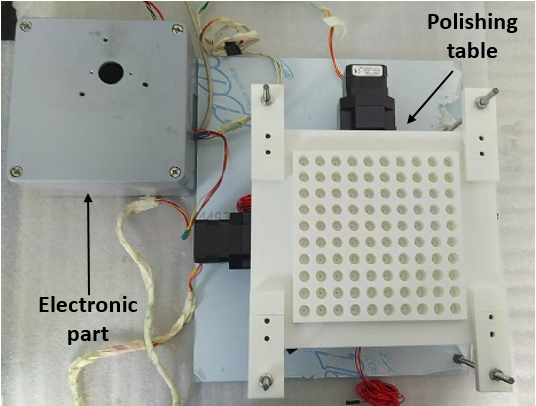
\includegraphics[angle=0, width=0.45\textwidth]{4ResearchAndDevelopments/41Fibers/GeneralViewPolishingMchine.png}}
    %\newline
  %\subfloat[Electronic system.]{
   %\label{subfig:ElectronicSystemPolishingMachine}
    %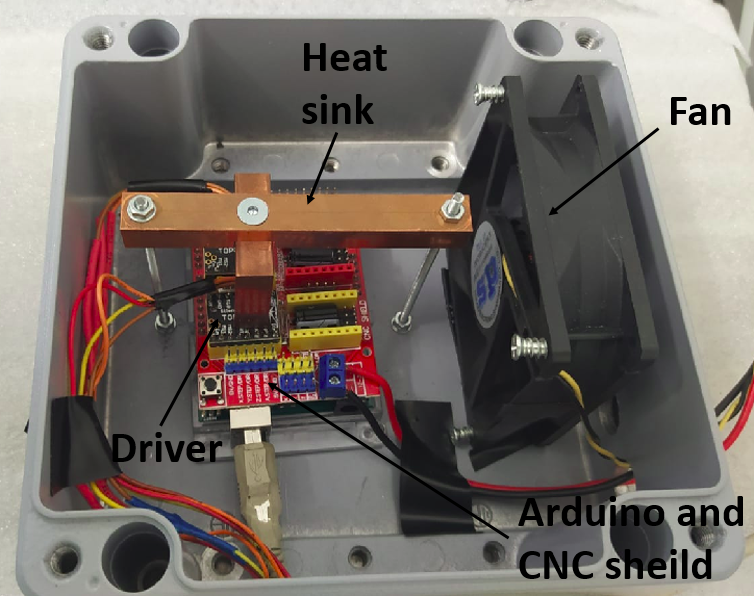
\includegraphics[angle=0, width=0.45\textwidth]{4ResearchAndDevelopments/41Fibers/ElectronicPolishingMachine.png}}
 %\caption{Polishing machine developed in TRITIUM experiment and the electronic system used.}
 %\label{fig:GeneralViewPolishingMachine}
%\end{figure}

\begin{figure}[h]
\centering
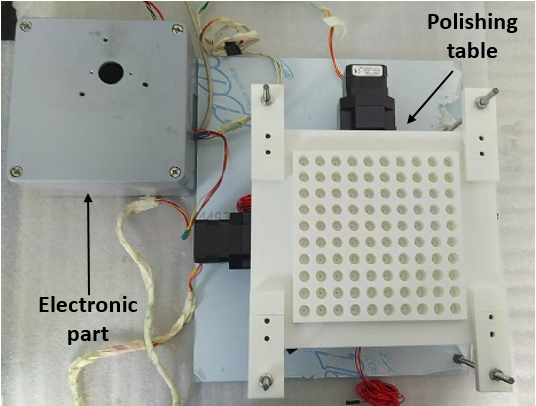
\includegraphics[scale=0.6]{4ResearchAndDevelopments/41Fibers/GeneralViewPolishingMchine.png}
\caption{Polishing machine developed in TRITIUM experiment.\label{fig:GeneralViewPolishingMachine}}
\end{figure}

As we can see in Figure \ref{fig:GeneralViewPolishingMachine}, this automatic polishing machine is based on two parts. On the one hand, the polishing table, where the fibers will be polished and, on the other hand, the electronics used, based on arduino technology, to automatically move the polishing table:

\begin{enumerate}
\item{} The polishing table can be divided in two parts, the immobile part, where the fibers will be fixed, and the mobile part, where the polishing papers will be fixed. We decided to move the polishing papers because they are lighter and mechanically easier than fibers.

The immobile part consists of a piece, shown in Figure \ref{subfig:PolishingTable}, which has been designed and built with a 3D printer, fixed to the system with four vertical screws. There are two nuts on each screw that are used to set the height and the inclination of fibers relative to the polishing papers. This piece contains one hundred holes where the fibers will be placed. 

Because of the reason that the fibers will press the polishing paper with their own weight, we use a plastic belt and a piece of metal with a weight of around $100~\gram$, shown in Figure \ref{subfig:FiberMetailcPiece}, to increase its weight (in the same way as in thorlabs polishing process).

The mobile part consists of a flat PMMA plate, whose dimensions are $18 \cdot{} 18~\cm^2$, on which the polishing paper will be fixed. This part is fixed to two horizontal screws, perpendicular to each other, that are used to move it around the XY plane (horizontal plane). This system is shown in Figure \ref{subfig:HorizontalAxis}.

This system contains multiple switches, each mounted on a piece designed with a 3D printer, shown in Figures \ref{subfig:PolishingTable}, \ref{subfig:HorizontalAxis} and \ref{subfig:3DSwitchPiece}. As we will see in this seciton, these switches are used to stop the system if they reach the end of the path and to find the coordinates origin.

\begin{figure}[htbp]
 \centering
  \subfloat[Polishing table.]{
   \label{subfig:PolishingTable}
    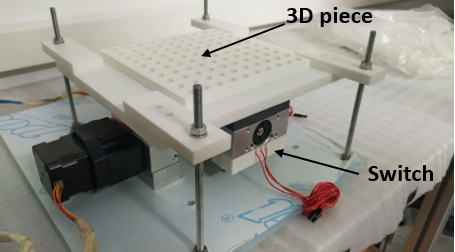
\includegraphics[angle=0, width=0.55\textwidth]{4ResearchAndDevelopments/41Fibers/PolishingTable.png}}
    %\newline
  \subfloat[Fiber with metal piece.]{
   \label{subfig:FiberMetailcPiece}
    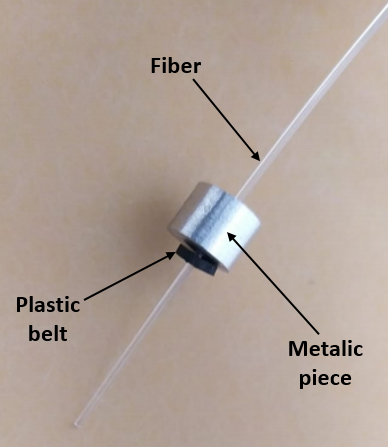
\includegraphics[angle=0, width=0.3\textwidth]{4ResearchAndDevelopments/41Fibers/PieceOfFiber.png}}
    \newline
   \subfloat[Horizontal screws and PMMA plate.]{
    \label{subfig:HorizontalAxis}
     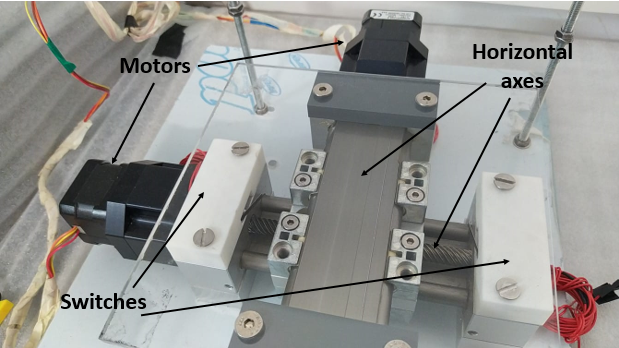
\includegraphics[angle=0, width=0.55\textwidth]{4ResearchAndDevelopments/41Fibers/HorizontalAxis2.png}}
     \subfloat[Piece to hold switches.]{
    \label{subfig:3DSwitchPiece}
     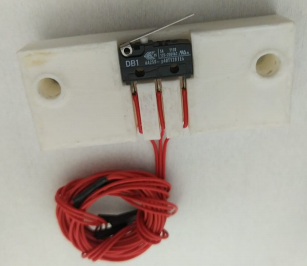
\includegraphics[angle=0, width=0.4\textwidth]{4ResearchAndDevelopments/41Fibers/Switch.png}}
 \caption{Polishing table of the polishing machine}
 \label{fig:PolishingTable}
\end{figure}

\item{} The electronic part, shown in Figure \ref{fig:ElectronicSystemPolishingMachine}, is based on arduino technology and it is used to achieve automatic movement of the polishing paper.

It consists of two stepper motors, model NEMA ST4209S1404-A \cite{StepperMotors}, which are used to control the horizontal screws on which the polishing paper is fixed. These motors are controlled by an arduino UNO \cite{ArduinoUNO} that uses a CNC shield \cite{CNCShield} in which two different drivers are connected to control these stepper motors, one driver for each stepper motor.

Drivers are controllers that allow you to manage stepper motors in a simple way. Choosing the correct controller for your system is very important because it can limit the supply power to the motors, causing the motors not to move in the worst case. Instead of using the Pololu A4988 drivers \cite{A4988Driver}, which is one of the most widely used drivers, our first choice was the DRV8825 driver \cite{DRV8825Driver} since DRV8825 allows to power the motor with higher voltage and intensities ($45~\volt$ and $2.5~\ampere$) than A4988 ($35~\volt$ and $2~\ampere$). Also, the DRV8825 controller includes a new microstepping mode ($1/32$) compared to the A4988 ($1/16$) with which we get more accurate and smooth movements.

Finally these drivers was replaced by the TMC2208 \cite{TMC2208Driver}. The main reason for this change was that they are much less noisy since it includes the \textit{StealthChop} function with which the noise is practically eliminated. On top of that, this controller is much more accurate as it has a microstepping mode of $1/256$.

The voltage and current used to power the motors are similar to the A4988 ($35~\volt$ and $2~\ampere$) which is sufficient for our system since the used motors are limited to $1.33~\ampere$. 

The excess current will be transformed into heat that we will have to dissipate from the system since overheating of these drivers can cause loss of steps, producing movements different from those programmed or even destroying the driver. Therefore, a cooling system is needed to ensure the correct operation of the polishing system.

The cooling system, shown in Figure \ref{fig:ElectronicSystemPolishingMachine}, is based on a fan and a copper piece\footnote{The copper is one of the best thermal conductor at STP} in contact with both controllers. It has the possibility to use a PELTIER cell to increase the cooling power of this system. A fan is also included to prevent heat accumulation inside the electronics box.

\begin{figure}[h]
\centering
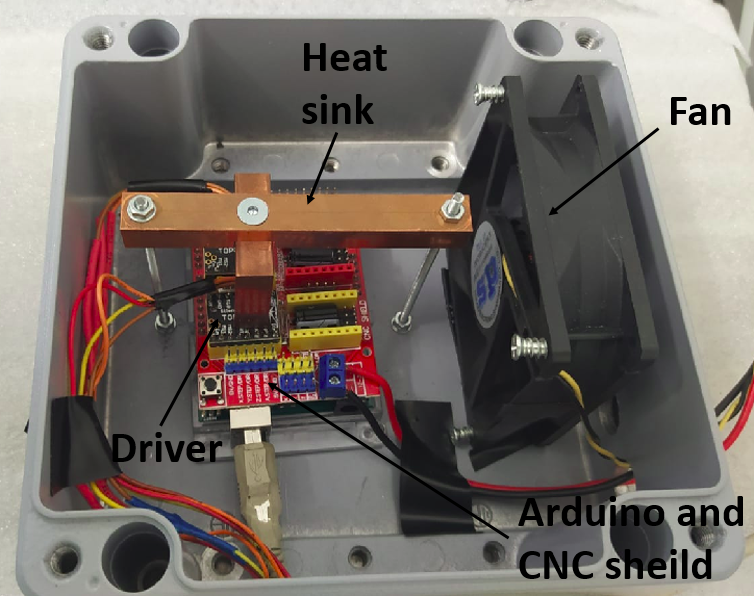
\includegraphics[scale=0.6]{4ResearchAndDevelopments/41Fibers/ElectronicPolishingMachine.png}
\caption{Electronic system of Polishing machine.\label{fig:ElectronicSystemPolishingMachine}}
\end{figure}

\end{enumerate}

This polishing machine is controlled by a computer using the Universal G-code Sender software (a grafical interface based on the GRBL package). It has several useful functions such as the "HOME" function with which the system, using the previously installed switches, finds its origin coordinate every time the system is turned on. 

It also has the ability to load a file containing the g-code to be executed, which is used for us to program the 120 movements required for each polishing paper.

To test this machine, tuenty fibers with a length of $15~\cm$ were cut and arranged in a bundle. They were fixed in a structure shown in Figure \ref{fig:BunchWith2PMTsCoincidence} with two PMTs located at their ends, which were read in time coincidence using the electronic system described in section \ref{subsubsec:PMTsElectronicalSystem}, Figure \ref{subfig:ElectronicConfiguraiton2PMT}.

\begin{figure}[]
\centering
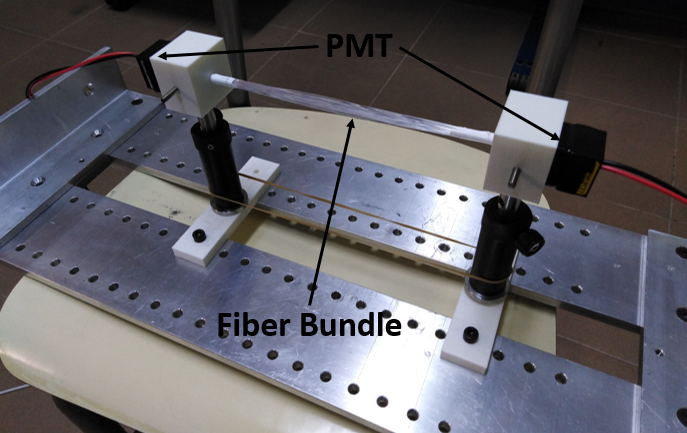
\includegraphics[scale=0.45]{4ResearchAndDevelopments/41Fibers/FiberBunch2PMTsCoincidence.png}
\caption{Set up used to test the effect of the polishing machine.\label{fig:BunchWith2PMTsCoincidence}}
\end{figure}

Two different measurements were taken using two different radioactive sources, $\ce{^{60}Co}$, whose activity was approximately $715~\becquerel$, as a gamma source and $\ce{^{90}Sr}$, whose activity was approximately $17.8~\kilo\becquerel$, as a beta source. After that, the fiber bundle was polished with the polishing machine developed and the test was repeated.

The energy spectrums recorded are shown in Figure \ref{fig:ResultsOfPolishingMachine} for each radioactive source, which where placed in the middle of the fiber, that's, $7.5~\cm$ from each PMT.

\begin{figure}[h]
 \centering
  \subfloat[Energy spectrum recorded for the Co-60 source.]{
   \label{subfig:EnergySpectrumCo60PolishingTest}
    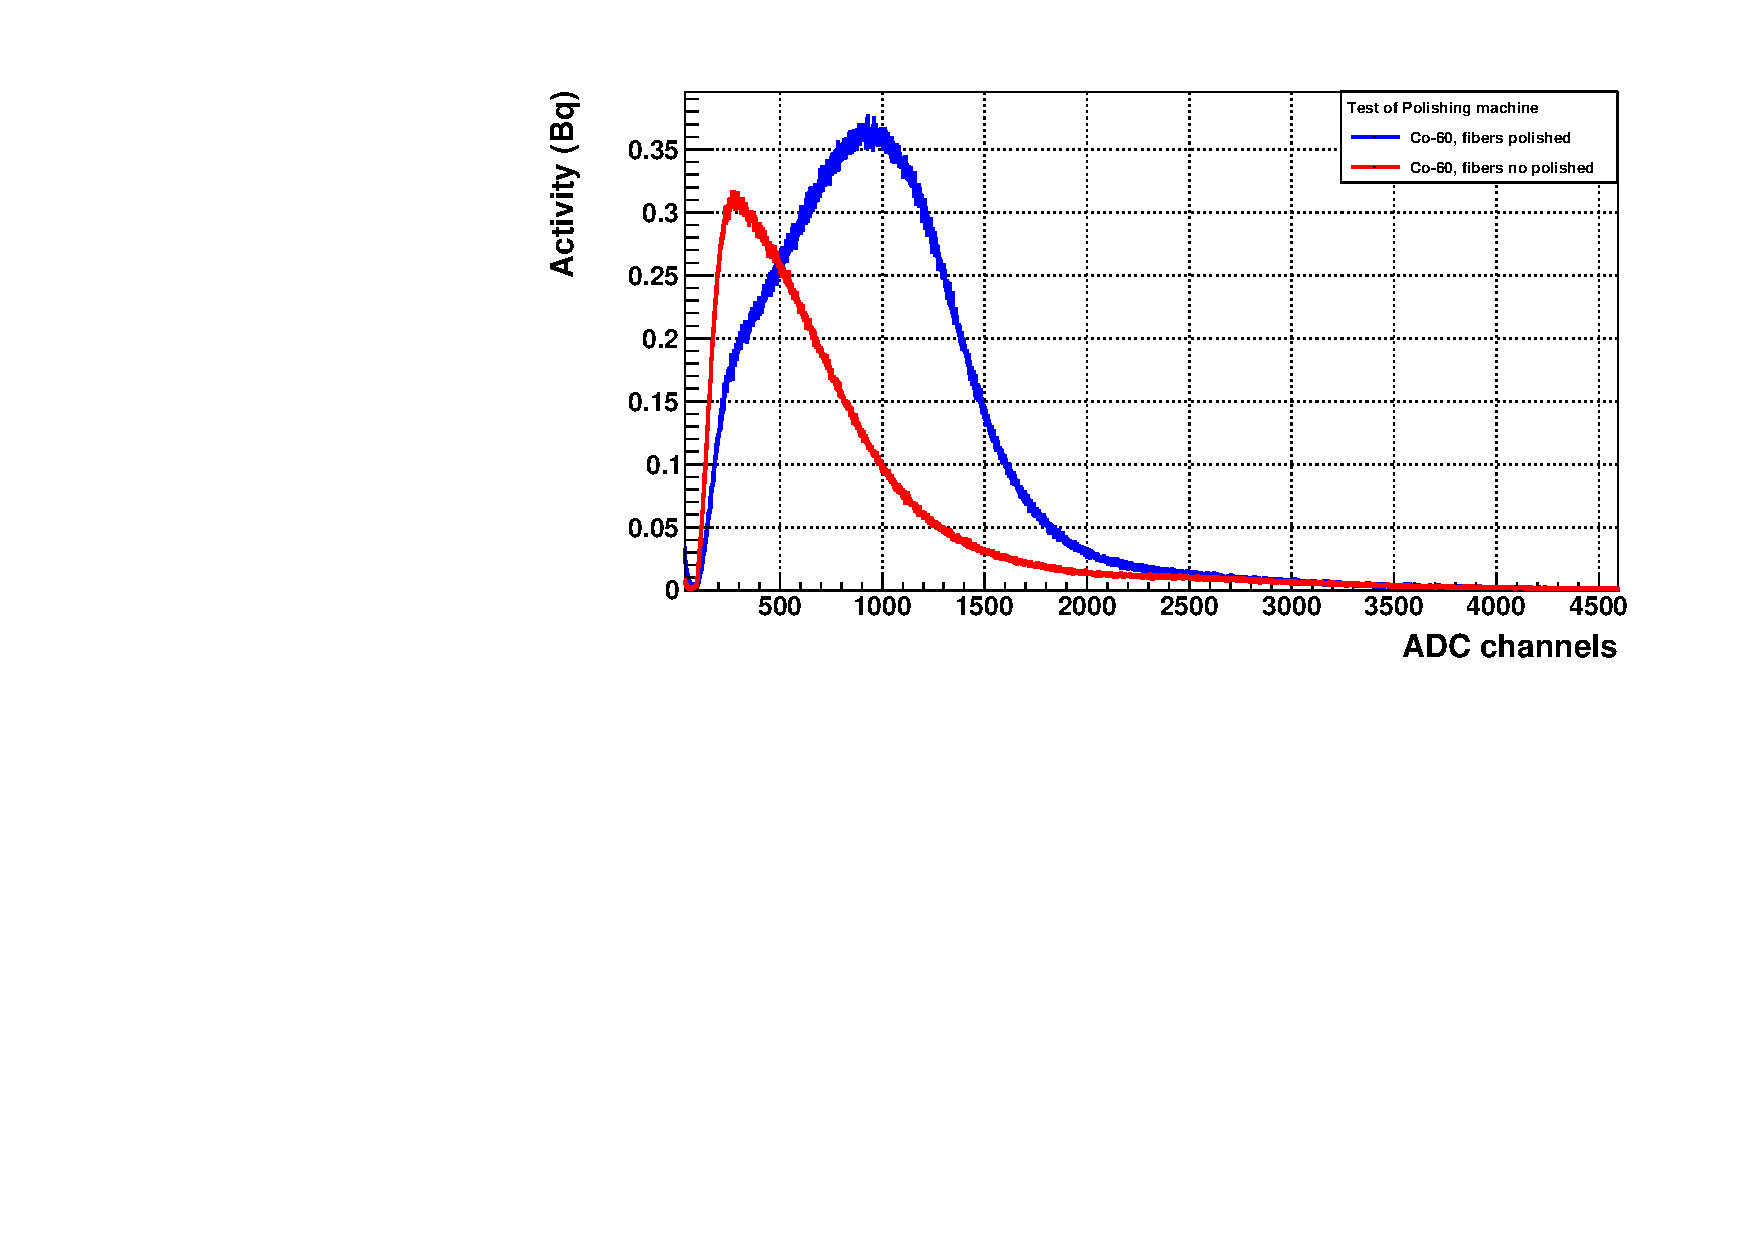
\includegraphics[width=0.76\textwidth]{4ResearchAndDevelopments/41Fibers/Co_60_PolishingMachine_ZOOM.pdf}}
    \newline
  \subfloat[Energy spectrum recorded for the Sr-90 source.]{
   \label{subfig:EnergySpectrumSr90PolishingTest}
    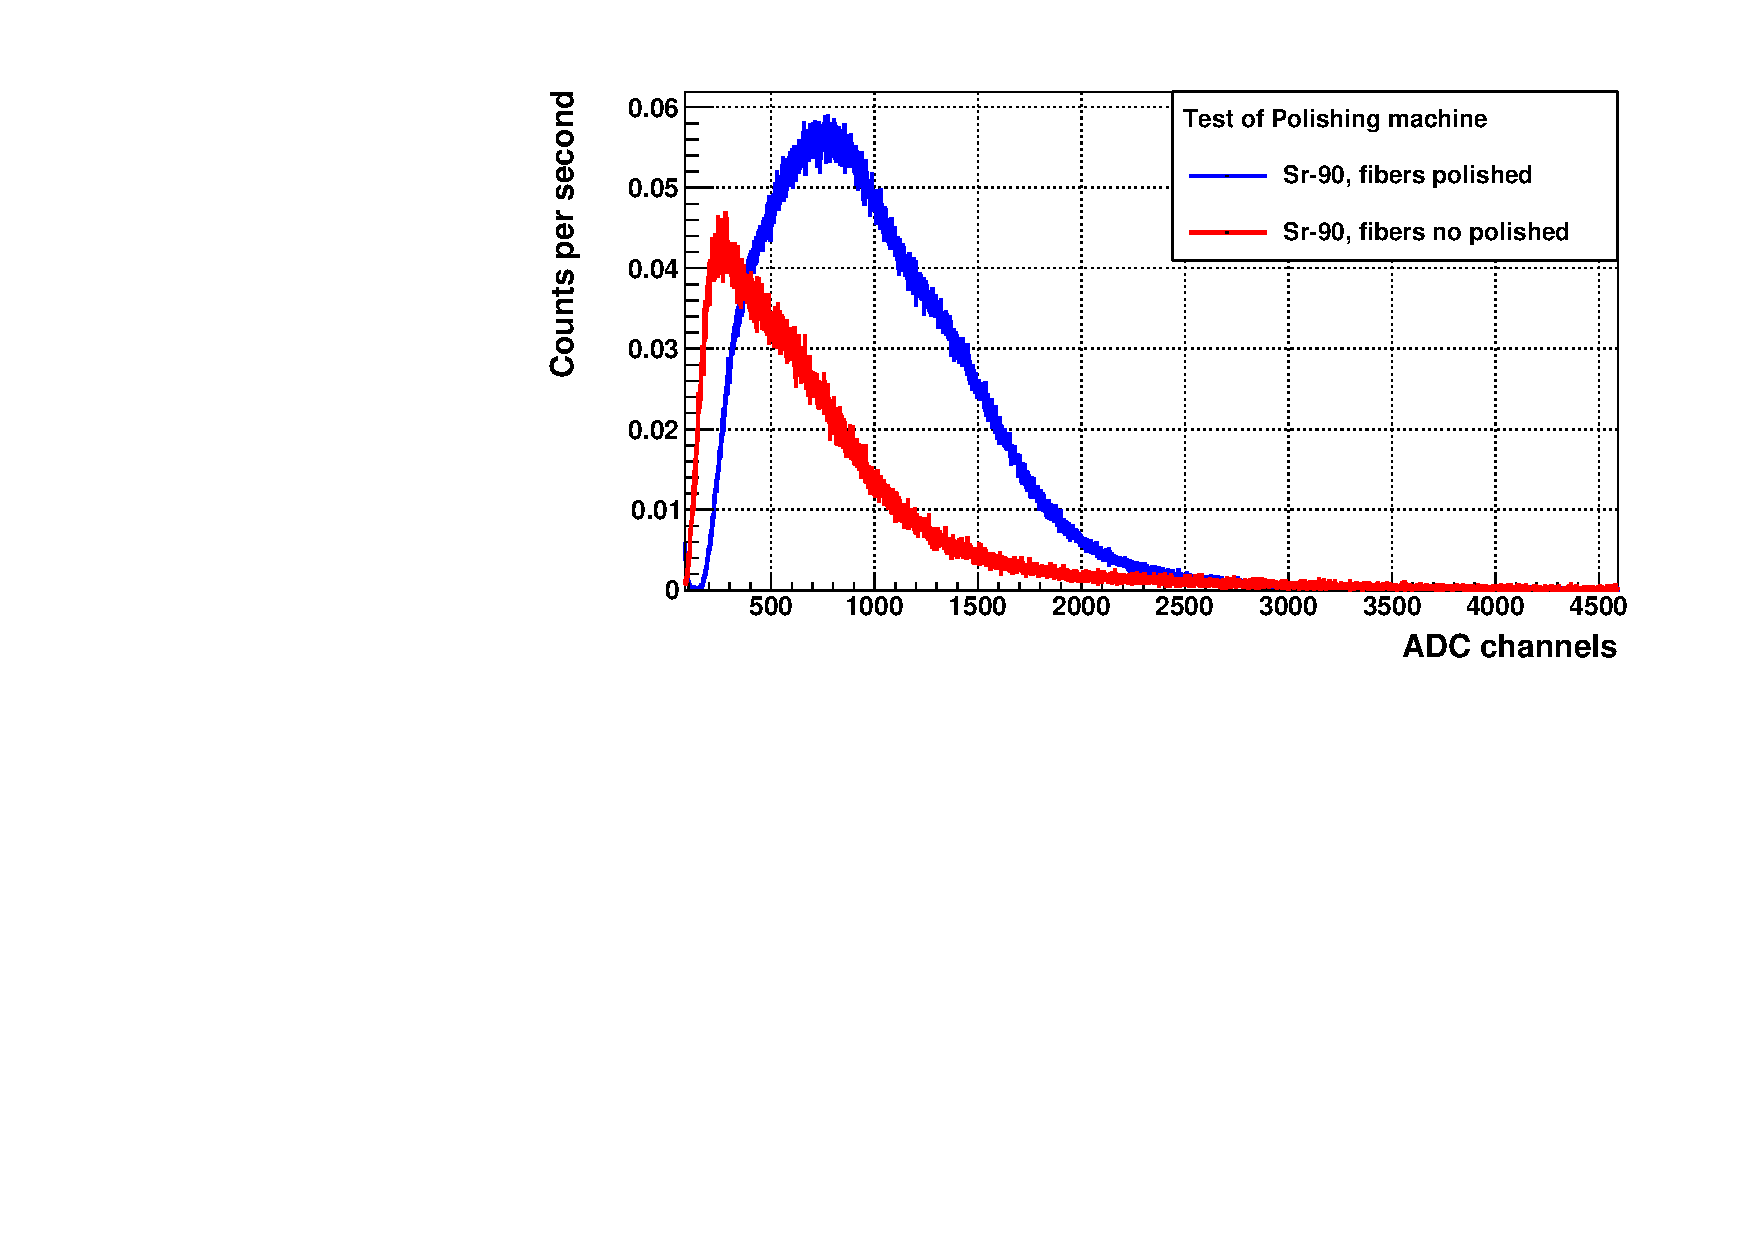
\includegraphics[width=0.76\textwidth]{4ResearchAndDevelopments/41Fibers/Sr_90_PolishingMchine_ZOOM.pdf}}
 \caption{Energy spectrums used to test the effect of the Polishing machine}
 \label{fig:ResultsOfPolishingMachine}
\end{figure}

As can be seen in these figures, both energy spectrums have shifted to the right of the spectrum, which means that the detected events have more energy (more photons per event has reached the PMTs). On top of that, an increase of more than 40\% (42\% for gamma source and 49\% for beta source) has been achieved in the number of counts registered in both cases.

The reason for this is that, with this process, we have improved the photon collection efficiency of the system (mainly because we have improved the interface between fibers and PMTs) which, as we discussed previously, is very important for the reason that we expect to detect few photons in each tritium event.